% Этот шаблон документа разработан в 2017 году
% Владимиром Коротковым (kvamob@mail.ru) 
%  

\documentclass[a4paper,12pt]{article} % добавить leqno в [] для нумерации слева

%% Глобальные Параметры страницы
\usepackage[left=3cm,right=2cm,top=1cm,bottom=2cm,bindingoffset=0cm]{geometry}

%\includeonly{O-41/h_granite.tex}

%\usepackage{fp} 						% Вычисления с плавающей точкой
%\usepackage{siunitx}					% При использовании пакета fp все числа должны иметь decimal delimiter точку
%\sisetup{output-decimal-marker={,}}	% Числа выводятся с запятой в качестве разделителя разрядов: \num{3.2} выводит 3,2 

%%% Работа с русским языком
\usepackage{cmap}					% поиск в PDF
\usepackage{mathtext} 				% русские буквы в формулах
\usepackage[T2A]{fontenc}			% кодировка
\usepackage[utf8]{inputenc}			% кодировка исходного текста
\usepackage[english,russian]{babel}	% локализация и переносы

%%% 
%\usepackage{rotating}				% Поворот текста

%%% Дополнительная работа с математикой
\usepackage{amsmath,amsfonts,amssymb,amsthm,mathtools} % AMS
\usepackage{icomma} % "Умная" запятая: $0,2$ --- число, $0, 2$ --- перечисление
\usepackage{gensymb}	% Градусы
%% Номера формул
%\mathtoolsset{showonlyrefs=true} % Показывать номера только у тех формул, на которые есть \eqref{} в  тексте.

%% Шрифты
\usepackage{euscript}	 % Шрифт Евклид
\usepackage{mathrsfs} % Красивый матшрифт


%% Перенос знаков в формулах (по Львовскому)
% \newcommand*{\hm}[1]{#1\nobreak\discretionary{}
%	{\hbox{$\mathsurround=0pt #1$}}{}}

%%% Работа с картинками
\usepackage{graphicx}  % Для вставки рисунков
%\usepackage[export]{adjustbox}
\graphicspath{{images/}}  % папки с картинками
\setlength\fboxsep{3pt} % Отступ рамки \fbox{} от рисунка
\setlength\fboxrule{0.2pt} % Толщина линий рамки \fbox{}
\usepackage{wrapfig} % Обтекание рисунков и таблиц текстом


%%% Работа с таблицами
\usepackage{array,tabularx,tabulary,booktabs} % Дополнительная работа с таблицами
\usepackage{longtable}  % Длинные таблицы
\usepackage{multirow} % Слияние строк в таблице

%%% Подписи к рисункам и таблицам в русской типографской традиции
\usepackage{caption} 
\DeclareCaptionFormat{GOSTtable}{#2#1\\#3}
\DeclareCaptionLabelSeparator{fill}{\hfill}
\DeclareCaptionLabelSeparator{dot}{. }
\DeclareCaptionLabelFormat{fullparents}{\bothIfFirst{#1}{~}#2}
\captionsetup[table]{
	format=GOSTtable,
	font={footnotesize},
	labelformat=fullparents,
	labelsep=fill,
	labelfont=rm,
%	labelfont=it,
	textfont=bf,
	justification=centering,
	singlelinecheck=false
}
\captionsetup{font=small}
\captionsetup[figure]{
	labelsep=dot, 
%	textfont=it
}
% А можно и так
%\captionsetup{labelsep=period}


%%% Модификация команд, задающих разделы
% Не подавлять отступы у первого абзаца

\makeatletter   % Команда \makeatletter делает символ @ буквой, команда \makeatother возвращает всё на свои места.
% Разрешим отступ у первого абзаца
\renewcommand\section{\@startsection {section}{1}{\parindent}%
	{3.5ex \@plus 1ex \@minus .2ex}{2.3ex \@plus.2ex}%
	{\normalfont\hyphenpenalty=10000\Large\bfseries}}

\renewcommand\subsection{\@startsection {subsection}{1}{\parindent}%
	{3.5ex \@plus 1ex \@minus .2ex}{2.3ex \@plus.2ex}%
	{\normalfont\hyphenpenalty=10000\large\bfseries}}
\makeatother

% После номеров разделов \section ставить точки
\usepackage{secdot}			
% И после \subsection тоже ставить точки
\sectiondot{subsection}		

\usepackage{lastpage} % Узнать, сколько всего страниц в документе.

\usepackage{soulutf8} % Модификаторы начертания

%\usepackage{hyperref}
%\usepackage[usenames,dvipsnames,svgnames,table,rgb]{xcolor}
%\hypersetup{				% Гиперссылки
%	unicode=true,           % русские буквы в раздела PDF
%	pdftitle={Заголовок},   % Заголовок
%	pdfauthor={Автор},      % Автор
%	pdfsubject={Тема},      % Тема
%	pdfcreator={Создатель}, % Создатель
%	pdfproducer={Производитель}, % Производитель
%	pdfkeywords={keyword1} {key2} {key3}, % Ключевые слова
%	colorlinks=true,       	% false: ссылки в рамках; true: цветные ссылки
%	linkcolor=red,          % внутренние ссылки
%	citecolor=green,        % на библиографию
%	filecolor=magenta,      % на файлы
%	urlcolor=cyan           % на URL
%}

\usepackage{multicol} % Несколько колонок

\usepackage{fancyhdr} % Колонтитулы
%\pagestyle{fancy}
%\renewcommand{\headrulewidth}{0mm}  % Толщина линейки, отчеркивающей верхний колонтитул
%\lfoot{Нижний левый}
%\rfoot{Нижний правый}
%\rhead{Верхний правый}
%\chead{Верхний в центре}
%\lhead{Верхний левый}
% \cfoot{Нижний в центре} % По умолчанию здесь номер страницы


%%%%%%%%%%%%%%%%%%%%%%%%%%%%%%%%%%%%%%%%%%%%%%%%%%%%%%%%%%%%%%%%%%%%%%%%%%%%%%%%%%%%%%%%%%%%%%%%%%%%%%%%%
%%% PAYLOAD
%%%%%%%%%%%%%%%%%%%%%%%%%%%%%%%%%%%%%%%%%%%%%%%%%%%%%%%%%%%%%%%%%%%%%%%%%%%%%%%%%%%%%%%%%%%%%%%%%%%%%%%%%

%%% Заголовок
\author{ООО <<Гидросфера>>}\label{company}
\title{ОТЧЕТ ПО РЕЗУЛЬТАТАМ ПОИСКОВ ИСТОЧНИКОВ ПОДЗЕМНЫХ ВОД}
\date{\today}
%%%======================================================================================================
\newcommand{\txtExecutor}{ООО <<Гидросфера>>}	% Исполнитель
\newcommand{\txtYear}{2019}						% Год
\newcommand{\txtAddress}{Челябинская область, р-н Каслинский, д Григорьевка, ул. Березовая, 3}			% Адрес
\newcommand{\txtCadaster}{74:09:0607001:633} 		% Кадастровый номер
\newcommand{\txtNomenclature}{O-41-31}	% Номенклатура листа М 1:200000
%\newcommand{\txtCoords}{56,162556	60,914785} % Координаты
%% ГИДРОГЕОЛОГИЧЕСКИЕ УСЛОВИЯ - Раскомментарить одно из:
\newcommand{\hydrogeology}{\textbf{Трещинные воды}. Уральская сложная гидрогеологическая складчатая область располагается в пределах орографически выраженного одноименного горно - складчатого сооружения. Основными коллекторами подземных вод являются трещиноватые породы коренного субстрата. Мощность зоны региональной трещиноватости составляет в среднем 30 – 100 м. Минимальные значения (20 – 30 м) присущи корам выветривания интрузивных пород; максимальные (60 – 100 м) – карбонатным породам; средние (40 – 60 м) – эффузивно-осадочным и метаморфическим комплексам. Помимо трещин выветривания широко развиты локальные линейные трещинные зоны высокой проницаемости и водоотдачи, связанные с проявлениями дизъюнктивной тектоники и контактами разнородных пород. Подземные воды региональной трещиноватости обычно гидравлически взаимосвязаны, имеют безнапорный характер и образуют небольшие бассейны с интенсивным
водообменном. В вертикальном разрезе фильтрационные свойства пород зоны выветривания неоднородны. По характеру их изменения зона разделяется на три части. В верхней (10 – 20 м), где широко представлены глины или суглинки элювиальной коры выветривания, водопроницаемые свойства очень низки; особенно широко коры распространены на площади Зауральского пенеплена. Средняя часть эрозионной зоны отличается наибольшей активностью, сильной степенью трещиноватости и высокой пористостью (от 1 до 7 \%). В нижней части размеры трещин весьма незначительны, и водоотдача пород практически отсутствует.

\textit{Водоносная зона трещиноватости позднепалеозойских интрузивных кислых и средних пород} ($\gamma PZ_3$) связана с массивами гранитов, гранодиоритов, плагиогранитов, диоритов. Региональная зона выветривания на этих массивах не превышает 15 – 20 м, зеркало подземных вод в сглаженной форме повторяет современный рельеф. Водоносность зоны крайне неравномерна: в центральных частях массивы практически безводны; по периферии (в приконтактовых частях с другими породами) водоносность возрастает до 0,2 – 0,3 л/с. В частности в тектонических и приконтактовых зонах позднепалеозойского Верхисетского гранитного массива отдельные скважины имели дебит до 7,0 л/с при удельном дебите 2,4 л/с, в центре массива оставаясь безводными. Минерализация вод – в пределах 0,08–0,5 г/дм\textsuperscript{3}; по составу преобладают гидрокарбонатные  кальциево-магниевые.

Гранодиориты и плагиограниты становятся более водоносными за счет секущих позднепалеозойских даек и жил «обновленных», к тому же тектоническими движениями создавшими условия для локализации трещинно-жильных вод в зоне выветривания. В окраинных частях Сысертского массива гранодиоритов и плагиогранитов дебиты скважин изменяются от 1,5 до 10,0 л/с при удельных дебитах 0,1 – 8,0 л/с. В центральной части (где нет жильных тел) в маломощной зоне выветривания дебиты скважин не превышают 0,3 – 0,5 л/с при удельных дебитах 0,001–0,01 л/с. Ближе к периферии фиксируютя мелкие источники с расходом 0,1 – 0,2 л/с. По минерализации и химическому составу воды аналогичны развитым в гранитных массивах. 

В целом питание подземных вод Большеуральского бассейна сезонное, за счет инфильтрации атмосферных осадков в теплый период года. Зеркало его вод в сглаженной форме повторяет основные элементы рельефа. На склонах и уплощенных водоразделах уровни воды залегают на глубинах 5 – 20 м, на хребтах и локальных возвышенностях – до 30 – 50 м. Сравнительно глубокая расчлененность дневной поверхности, особенно в районах приподнятых горных массивов, обеспечивает хорошие условия дренирования водоносных зон речной сетью. Разгрузка вод идет преимущественно вдоль долин рек, а также может быть приурочена к локальным трещинным зонам. Дебиты родников, в зависимости от величины водосборной площади, варьируют от долей до многих десятков литров в секунду.

Эксплуатационные ресурсы Большеуральского бассейна связываются преимущественно с крупными карбонатными массивами среднего и верхнего палеозоя и тектонически активными зонами разломов, на которых возможна организация водозаборов с дебитом 100 – 1000 л/с. На остальных водоносных зонах трещиноватости возможен каптаж подземных вод по отдельным кустам скважин с дебитами от 10 до 30 л/с. Ресурсы порово-пластовых вод Иртыш-Обского бассейна связаны преимущественно с опоковым горизонтом палеоцена, мощность обводненной толщи которого 3 – 4 м на западе и до 50 м на востоке. На придолинных участках некоторые водозаборы из него имеют производительность до 50–100 л/с.

Несмотря на значительное количество водоносных горизонтов на изученной площади, наиболее промышленные и обжитые районы Урала испытывают недостаток в водообеспеченности из-за неравномерного распределения ресурсов, а также в связи с невозможностью создания крупных водозаборов с высокой производительностью на локальных участках водоносных зон.
}			% Гранитные интрузии
%\newcommand{\hydrogeology}{\textbf{Трещинные воды}. Уральская сложная гидрогеологическая складчатая область располагается в пределах орографически выраженного одноименного горно - складчатого сооружения. Основными коллекторами подземных вод являются трещиноватые породы коренного субстрата. Мощность зоны региональной трещиноватости составляет в среднем 30  --  100~м. Минимальные значения (20  --  30~м) присущи корам выветривания интрузивных пород; максимальные (60  --  100~м)  --  карбонатным породам; средние (40  --  60~м)  ---  эффузивно-осадочным и метаморфическим комплексам. Помимо трещин выветривания широко развиты локальные линейные трещинные зоны высокой проницаемости и водоотдачи, связанные с проявлениями дизъюнктивной тектоники и контактами разнородных пород. Подземные воды региональной трещиноватости обычно гидравлически взаимосвязаны, имеют безнапорный характер и образуют небольшие бассейны с интенсивным
водообменном. В вертикальном разрезе фильтрационные свойства пород зоны выветривания неоднородны. По характеру их изменения зона разделяется на три части. В верхней (10  --  20~м), где широко представлены глины или суглинки элювиальной коры выветривания, водопроницаемые свойства очень низки; особенно широко коры распространены на площади Зауральского пенеплена. Средняя часть эрозионной зоны отличается наибольшей активностью, сильной степенью трещиноватости и высокой пористостью (от 1 до 7~\%). В нижней части размеры трещин весьма незначительны, и водоотдача пород практически отсутствует.

\textit{Водоносная зона трещиноватости средне-верхнепалеозойских карбонатных образований} ($сPZ_{2–3}$) является одной из наиболее водообильных. Она развита преимущественно в пределах синклинальных, реже антиклинальных структурных форм в виде отдельных разобщенных либо взаимосвязанных между собой водоносных горизонтов меридионального и субмеридионального простирания. Наиболее изученные Невьянская, Алапаевская,
Каменская зоны имеют площади до 200 км\textsuperscript{2}. Водовмещающими породами являются известняки с пачками и прослоями глинистых сланцев, аргиллитов, песчаников и туффитов. Трещиновато-карстовая зона имеет мощность 50  --  80~м, достигая в зонах тектонических нарушений 200  --  250~м. С поверхности карбонатные породы осложнены проявлениями карста (в виде воронок); в пределах мезозойских депрессий карст перекрыт кайнозойскимиотложениями, мощность до 20  --  30~м.

Карстовым процессам подвержены все карбонатные «массивы», но степень их проявления неравномерна. На Алапаевском «массиве» скважинами выявлены погребенные щелевидные депрессии длиной до 900  --  2000~м
при ширине 400  --  500~м и глубиной от 70 до 140~м в осевой части.

Характерной особенностью древних карстовых депрессий является высокая трещиноватость бортовых частей и слабая водонасыщенность днищ. Погребенные карстово - трещинные воды в депрессиях обладают напором, соответствующим мощности экранирующего покрова. Питание подземных вод осуществляется за счет инфильтрации атмосферных осадков и разгрузки сопряженных вод из других горизонтов. Циркуляция происходит по сложному лабиринту карстовых пустот и трещин, коэффициент фильтрации в которых варьирует от 2  --  5 до 30~м/сут. Максимальная водообильность приурочена к придолинным участкам пересечения с линейными водоносными зонами. Дебиты родников в них достигают 10  --  25~л/с; в стороне от речных долин вне водоносных зон дебиты не превышают 3  --  5~л/с. Химический состав и минерализация трещинно-карстовых вод изменяются в меридиональном направлении: до широты г. Алапаевск преобладают гидрокарбонатные кальциевые, реже кальциево-магниевые воды с минерализацией от 0,1 до 0,4 г/дм\textsuperscript{3}; южнее распространены гидрокарбонатные кальциево-магниевые, реже кальциевые воды с минерализацией от 0,2 до 0,6 -- 0,8 г/дм\textsuperscript{3}.

В целом питание подземных вод Большеуральского бассейна сезонное, за счет инфильтрации атмосферных осадков в теплый период года. Зеркало его вод в сглаженной форме повторяет основные элементы рельефа. На склонах и уплощенных водоразделах уровни воды залегают на глубинах 5  --  20~м, на хребтах и локальных возвышенностях  ---  до 30  --  50~м. Сравнительно глубокая расчлененность дневной поверхности, особенно в районах приподнятых горных массивов, обеспечивает хорошие условия дренирования водоносных зон речной сетью. Разгрузка вод идет преимущественно вдоль долин рек, а также может быть приурочена к локальным трещинным зонам. Дебиты родников, в зависимости от величины водосборной площади, варьируют от долей до многих десятков литров в секунду.

Эксплуатационные ресурсы Большеуральского бассейна связываются преимущественно с крупными карбонатными массивами среднего и верхнего палеозоя и тектонически активными зонами разломов, на которых возможна организация водозаборов с дебитом 100  --  1000~л/с. На остальных водоносных зонах трещиноватости возможен каптаж подземных вод по отдельным кустам скважин с дебитами от 10 до 30~л/с. Ресурсы порово-пластовых вод Иртыш-Обского бассейна связаны преимущественно с опоковым горизонтом палеоцена, мощность обводненной толщи которого 3  --  4~м на западе и до 50~м на востоке. На придолинных участках некоторые водозаборы из него имеют производительность до 50 -- 100~л/с.

Несмотря на значительное количество водоносных горизонтов на изученной площади, наиболее промышленные и обжитые районы Урала испытывают недостаток в водообеспеченности из-за неравномерного распределения ресурсов, а также в связи с невозможностью создания крупных водозаборов с высокой производительностью на локальных участках водоносных зон.
}		% Карбонтаные образования 
%\newcommand{\hydrogeology}{\textbf{Трещинные воды}. Уральская сложная гидрогеологическая складчатая область располагается в пределах орографически выраженного одноименного горно - складчатого сооружения. Основными коллекторами подземных вод являются трещиноватые породы коренного субстрата. Мощность зоны региональной трещиноватости составляет в среднем 30  --  100~м. Минимальные значения (20  --  30~м) присущи корам выветривания интрузивных пород; максимальные (60  --  100~м)  ---  карбонатным породам; средние (40  --  60~м)  ---  эффузивно-осадочным и метаморфическим комплексам. Помимо трещин выветривания широко развиты локальные линейные трещинные зоны высокой проницаемости и водоотдачи, связанные с проявлениями дизъюнктивной тектоники и контактами разнородных пород. Подземные воды региональной трещиноватости обычно гидравлически взаимосвязаны, имеют безнапорный характер и образуют небольшие бассейны с интенсивным водообменном. В вертикальном разрезе фильтрационные свойства пород зоны выветривания неоднородны. По характеру их изменения зона разделяется на три части. В верхней (10  --  20~м), где широко представлены глины или суглинки элювиальной коры выветривания, водопроницаемые свойства очень низки; особенно широко коры распространены на площади Зауральского пенеплена. Средняя часть эрозионной зоны отличается наибольшей активностью, сильной степенью трещиноватости и высокой пористостью (от 1 до 7 \%). В нижней части размеры трещин весьма незначительны, и водоотдача пород практически отсутствует.

\textit{Водоносная зона трещиноватости нижнепалеозойских ультраосновных пород} ($\Sigma PZ_1$)
связана с перидотитами, дунитами и полнопроявленными серпентинитами, образующими в рельефе значительные возвышенности субмеридионального простирания с ограниченными бассейнами питания трещинных грунтовых вод. Породы весьма устойчивы к процессам выветривания; мощности трещиноватой зоны не превышают 10  --  15~м. В центральных частях массивы практически безводны, а в окраинных расход родников варьирует от 0,01 до 0,2  --  0,3~л/с. Дебиты скважин, вскрывших выветрелые трещиноватые серпентиниты, не превышают 1,5 -- 2,5~л/с.

Наибольшая обводненность приурочена к периферийным разломам, обновленным неотектоникой. В частности, по отдельным данным, восточная часть Колинского серпентинитового массива (в районе г. Серов) «срезана» в плане и опущена на 200~м региональным ступенчатым сбросом, прослеживаемым на 150 км. Вдоль этого нарушения ультрамафиты трещиноваты и аккумулируют подземный сток грунтовых вод зоны выветривания. Дебиты
скважин в этой зоне изменяются от 5 до 30~л/с при удельных дебитах 0,5  --  6,5~л/с. По периферии других массивов водоносность нередко связана с жилами и дайками кислого и основного составов, имеющими более молодой возраст. Грунтово-трещинные и трещинно-жильные воды имеют минерализацию 0,1 -- 0,5 г/дм\textsuperscript{3}, и лишь на отдельных массивах встречаются ультрапресные воды. По химическому составу они гидрокарбонатные магниевые или гидрокарбонатные магниево-кальциевые. Высокие показатели магния обусловлены большим содержанием его окиси в коренных породах.

Водоносные горизонты зон высокой проницаемости и водоотдачи приурочены к омоложенным в новейшее время дизъюнктивам. Детально одна из таких тектонических зон была изучена А. В. Скалиным в Екатеринбурге
при инженерно-геологических изысканиях под высотные здания в центре города. Она приурочена к контакту габбрового массива с вулканогенной толщей и имеет ширину до 60~м. Коэффициент фильтрации здесь составляет 10  --  20~м/сут (трещиноватое габбро  --  до 1~м/сут). При опытных откачках дебит скважин в трещиноватых габбро не превышает 1,4 дм\textsuperscript{3}/с, в тектонической зоне  ---  3,5 дм\textsuperscript{3}/с. Суммарный дебит последней по кустовой откачке трех скважин составил 950~м\textsuperscript{3}/сут.

В целом питание подземных вод Большеуральского бассейна сезонное, за счет инфильтрации атмосферных осадков в теплый период года. Зеркало его вод в сглаженной форме повторяет основные элементы рельефа. На склонах и уплощенных водоразделах уровни воды залегают на глубинах 5  --  20~м, на хребтах и локальных возвышенностях  ---  до 30  --  50~м. Сравнительно глубокая расчлененность дневной поверхности, особенно в районах приподнятых горных массивов, обеспечивает хорошие условия дренирования водоносных зон речной сетью. Разгрузка вод идет преимущественно вдоль долин рек, а также может быть приурочена к локальным трещинным зонам. Дебиты родников, в зависимости от величины водосборной площади, варьируют от долей до многих десятков литров в секунду.

Эксплуатационные ресурсы Большеуральского бассейна связываются преимущественно с крупными карбонатными массивами среднего и верхнего палеозоя и тектонически активными зонами разломов, на которых возможна организация водозаборов с дебитом 100  --  1000~л/с. На остальных водоносных зонах трещиноватости возможен каптаж подземных вод по отдельным кустам скважин с дебитами от 10 до 30~л/с. Ресурсы порово-пластовых вод Иртыш-Обского бассейна связаны преимущественно с опоковым горизонтом палеоцена, мощность обводненной толщи которого 3  --  4~м на западе и до 50~м на востоке. На придолинных участках некоторые водозаборы из него имеют производительность до 50 -- 100~л/с.

Несмотря на значительное количество водоносных горизонтов на изученной площади, наиболее промышленные и обжитые районы Урала испытывают недостаток в водообеспеченности из-за неравномерного распределения ресурсов, а также в связи с невозможностью создания крупных водозаборов с высокой производительностью на локальных участках водоносных зон.
}	% Гипербазиты, серпентиниты и габбро
%\newcommand{\hydrogeology}{\textbf{Трещинные воды}. Уральская сложная гидрогеологическая складчатая область располагается в пределах орографически выраженного одноименного горно - складчатого сооружения. Основными коллекторами подземных вод являются трещиноватые породы коренного субстрата. Мощность зоны региональной трещиноватости составляет в среднем 30 – 100 м. Минимальные значения (20 – 30 м) присущи корам выветривания интрузивных пород; максимальные (60 – 100 м) – карбонатным породам; средние (40 – 60 м) – эффузивно-осадочным и метаморфическим комплексам. Помимо трещин выветривания широко развиты локальные линейные трещинные зоны высокой проницаемости и водоотдачи, связанные с проявлениями дизъюнктивной тектоники и контактами разнородных пород. Подземные воды региональной трещиноватости обычно гидравлически взаимосвязаны, имеют безнапорный характер и образуют небольшие бассейны с интенсивным водообменном. В вертикальном разрезе фильтрационные свойства пород зоны выветривания неоднородны. По характеру их изменения зона разделяется на три части. В верхней (10 – 20 м), где широко представлены глины или суглинки элювиальной коры выветривания, водопроницаемые свойства очень низки; особенно широко коры распространены на площади Зауральского пенеплена. Средняя часть эрозионной зоны отличается наибольшей активностью, сильной степенью трещиноватости и высокой пористостью (от 1 до 7 \%). В нижней части размеры трещин весьма незначительны, и водоотдача пород практически отсутствует.

\textit{Водоносная зона трещиноватости палеозойских вулканогенно - осадочных и метаморфических образований} ($an, gsPR_1–PZ$) представлена эффузивами различного состава и их туфами, туфоконгломератами и туфопесчаниками различного состава при участии метаморфических зеленых аповулканогенных и глинисто-кремнистых сланцев, слюдяных кристаллосланцев, прослоями метапесчаников и метаморфизованных известняков. Вулканогенные породы и метаморфиты обладают близкими коллекторскими свойствами; подземные воды в них приурочены к грубообломочным и карбонатным прослоям, а также к зонам трещиноватости тектонического происхождения. 

Фильтрационное поле метаморфических пород расчленяется на серию гидравлически связанных и вытянутых по простиранию блоков шириной от десятков до первых километров, структура которых имеет мозаичный характер, обусловленный сочетанием трещин регионального выветривания, разломов и линейных слабопроницаемых экранов. Водоносная трещиноватая зона прослеживается до глубин от 30 до 100 м, преобладающие значения – до 40 – 60 м.

Наиболее глубоко она проникает в горной (открытой) части Уральского складчатого сооружения; близко от поверхности фиксируется в тектонически ослабленных зонах и в долинах рек. На площади Зауральского пенеплена водоносный горизонт перекрыт глинистой корой выветривания и имеет напорный характер до 10–15 м. Водопритоки в скважины составляют от 0,1 – 0,5 до 2 – 3 л/с; в локальных трещинах – в 5–10 раз выше. Дебиты родников в доли нах рек варьируют от 0,5 до 15 – 20 л/с (средний расход 0,8 л/с).
Высокой водообильностью обладают жильные тела, секущие вулканогенно-осадочные породы: дебиты скважин в них составляют 2–3 л/с. На Березовском золоторудном поле, которое представляет собой огромное скопление жил (площадью около 75 км\textsuperscript{2}), шахтный водоотлив в годы наиболее интенсивных горных работ составлял 500 – 600 м\textsuperscript{3}/ч. Питание подземных вод происходит за счет атмосферных осадков; по химическому составу воды гидрокарбонатные кальциево-магниевые, с минерализацией 0,2 – 0,6 г/дм\textsuperscript{3}.

В целом питание подземных вод Большеуральского бассейна сезонное, за счет инфильтрации атмосферных осадков в теплый период года. Зеркало его вод в сглаженной форме повторяет основные элементы рельефа. На склонах и уплощенных водоразделах уровни воды залегают на глубинах 5 – 20 м, на хребтах и локальных возвышенностях – до 30 – 50 м. Сравнительно глубокая расчлененность дневной поверхности, особенно в районах приподнятых горных массивов, обеспечивает хорошие условия дренирования водоносных зон речной сетью. Разгрузка вод идет преимущественно вдоль долин рек, а также может быть приурочена к локальным трещинным зонам. Дебиты родников, в зависимости от величины водосборной площади, варьируют от долей до многих десятков литров в секунду.

Эксплуатационные ресурсы Большеуральского бассейна связываются преимущественно с крупными карбонатными массивами среднего и верхнего палеозоя и тектонически активными зонами разломов, на которых возможна организация водозаборов с дебитом 100 – 1000 л/с. На остальных водоносных зонах трещиноватости возможен каптаж подземных вод по отдельным кустам скважин с дебитами от 10 до 30 л/с. Ресурсы порово-пластовых вод Иртыш-Обского бассейна связаны преимущественно с опоковым горизонтом палеоцена, мощность обводненной толщи которого 3 – 4 м на западе и до 50 м на востоке. На придолинных участках некоторые водозаборы из него имеют производительность до 50–100 л/с.

Несмотря на значительное количество водоносных горизонтов на изученной площади, наиболее промышленные и обжитые районы Урала испытывают недостаток в водообеспеченности из-за неравномерного распределения ресурсов, а также в связи с невозможностью создания крупных водозаборов с высокой производительностью на локальных участках водоносных зон.
}		% Вулканогенно-осад. и метаморф.
% Легенда
%\newcommand{\txtLegendFname}{Legend-o-41-25.jpg}				% Легенда - имя файла
%\newcommand{\txtLegendFname}{Legend-o-41-26.jpg}				% Легенда - имя файла
\newcommand{\txtLegendFname}{Legend-o-41-31.jpg}				% Легенда - имя файла
%\newcommand{\txtLegendFname}{Legend-o-41-32.jpg}				% Легенда - имя файла

%%
% Геологические условия
\def\txtGeology{
	В геологическом  отношении площадка  сложена  \textit{мраморизованными известняками, контактирующими к востоку с гранитами}. Скальные породы в~верхней зоне сильно выветрелые и разбиты трещинами.
}
% Результаты рекогносцировочных работ
\def\txtRecog{
	Изучаемый участок расположен по~адресу: \txtAddress .
	В номенклатуре топографических планшетов участок расположен на~листе \textbf{O-41-XXXI} масштаба \textbf{1:200000}. 
	
	\txtGeology
	
	Верхняя часть разреза сложена слабопроницаемыми грунтами, поэтому существует реальная угроза подтопления зданий и~сооружений и~заболачивания участка. Осложняющим фактором при бурении является приуроченность участка к~тектонической зоне.
	
	В геоморфологическом отношении рассматриваемый участок находится неподалеку от северного берега оз. Анжелы.
	Трещинные и трещинно-жильные подземные воды в пределах участка формируются на залесенных возвышенностях в окрестностях поселка за счет инфильтрации атмосферных осадков.
}
% Камеральные работы
\def\txtCamer{
	\begin{itemize}
		\item в~пределах перспективного участка выделена серия водоносных зон сосредоточенной разгрузки подземных вод.
		\item Наличие трещиноватых зон на~глубине от 24~м в~месте сосредоточенной разгрузки подземных вод.
		\item Мощность выявленных водоносных зоны 0,5~м, простирание -- до~1,5 -- 2,0 ~км.
		\item Место заложения скважины водоснабжения рекомендуется выбирать \textbf{в пределах узлов пересечения выявленных водоносных зон}.
	\end{itemize}
}
% Рекомендации
\def\txtRecommend{
	\begin{itemize}
		\item Для обеспечения требуемых потребностей в~воде рекомендуется проходка скважины водоснабжения в~пределах узлов пересечения выявленных водоносных зон сосредоточенной разгрузки подземных вод. Ориентировочная глубина скважины в~этом случае составит порядка 30~м.
		\item Положение скважины будет помечено на~местности репером.
		\item Обсадку трубами беcщелевой перфорации целесообразно выполнить  до~коренных грунтов на~глубину до~22 - 25~м от поверхности земли.
		\item Во избежание попадания верховодки целесообразно применять обсадку трубами до~глубины 5 -- 8~м. 
		\item Крайне не рекомендуется устройство заглублений вокруг устья скважины, для отвода воды из~скважины необходимо использовать \textbf{водопровод  незаглубленного типа}, так как водопроводная траншея по~сути является дренажной канавой, собирающей в~себя поверхностные воды и~«верховодку» далеко не лучшего качества, которые к~тому же вымывают песок из~суглинков, далее эти загрязненные воды с песком по~затрубному пространству поступают в~скважину, вызывая загрязнение и~запесочивание скважины.
	\end{itemize}
}


%%%%%%%%%%%%%%%%%%%%%%%%%%%%%%%%%%%%%%%%%%%%%%%%%%%%%%%%%%%%%%%%%%%%%%%%%%%%%%%%%%%%%%%%%%%%%%%%%%%%%%%%%

\begin{document} % конец преамбулы, начало документа

\setlength{\extrarowheight}{1mm} % Дополнительный интервал между строками таблиц

%% Титульная страница

\begin{titlepage}
	\begin{center}
		\textbf{\txtExecutor}
		\vspace{7.5cm}
		
		{\LARGE ОТЧЕТ ПО РЕЗУЛЬТАТАМ ПОИСКОВ}

		\bigskip

		{\LARGE ИСТОЧНИКОВ ПОДЗЕМНЫХ ВОД}
		
		\bigskip
		
		на участке по~адресу:
		\bigskip
				
		\underline{\txtAddress}
		
		\bigskip
		Кадастровый номер \txtCadaster
		
		\vfill
	
		\bigskip
		
	\end{center}

	\vfill
	
	\newlength{\ML}
	\settowidth{\ML}{«\underline{\hspace{0.7cm}}» \underline{\hspace{2cm}}}
	\hfill
	\begin{minipage}{1.0\textwidth}
		Директор ООО <<Гидросфера>> к.г.м.н.
		\underline{\hspace{\ML}} А.\,А.~Кашкаров\\
	\end{minipage}%
	
	\bigskip
	
	\vfill
	\begin{center}
		Екатеринбург, \txtYear
	\end{center}			

	\end{titlepage}

%%%%%%%%%%%%%%%%%%%%%%%%%%%%%%%%%%%%%%%%%%%%%%%%%%%%%%%%%%%%%%%%%%%%%%%%%%%%%%%%%%%%%%%%%%%%%%%%%%%%%%%%%%%%%%%%%%%%%%%%%%
\tableofcontents

\listoffigures

% \listoftables

\bigskip

%\textbf{ПРИЛОЖЕНИЯ}

\newpage
%%%%%%%%%%%%%%%%%%%%%%%%%%%%%%%%%%%%%%%%%%%%%%%%%%%%%%%%%%%%%%%%%%%%%%%%%%%%%%%%%%%%%%%%%%%%%%%%%%%%%%%%%%%%%%%%%%%%%%%%%%

\section{Введение}

Изыскания источников подземных вод -- важнейший этап в~производстве комплексных работ по~водоснабжению землепользователей за счет источников подземных вод, основанный изучении миграции подземных вод к~местам их разгрузки.

Круговорот воды в~природе чаще всего воспринимается как сток поверхностных вод к~морям и~океанам. Однако согласно статистическим сведениям, под землей хранится и~перемещается на~порядок больший объем воды, чем в~реках и~ручьях.

Теоретические и~практические работы, выполненные автором настоящего заключения, убедительно показали, что участки земной коры, в~которых наблюдается эффективная фильтрация подземной воды, имеют в~поперечнике размер от 0,5 до~1,0~метра, по~протяженности более 2~км, по~глубине не превышает высоту изучаемого участка над уровнем моря. Такие участки наиболее перспективны для организации водозаборов. Именно они являются объектом изысканий, поскольку при минимальной глубине из~них можно получить максимальный объем воды наиболее высокого качества. Качество воды определяется ее высокой обновляемостью в~водоносных зонах, исключающую застойность, высокую минерализацию и~жесткость.

Методы изысканий предполагают использование комплекса электроразведочных работ и~оригинальный метод интерпретации, связанный с трансформацией геоэлектрических моделей грунтов в~гидрогеологические и~геомеханические модели.

\section{Цель изыскательских работ}
Целью выполненного комплекса изыскательских работ являются:
\begin{itemize}
	\item изучение геологического строения верхней части земной коры, литологии, стратиграфии процессов выветривания, техногенного изменения, тектоники и~т.д.
	\item гидрогеологических условий верхней части земной коры с точки зрения фильтрационных возможностей грунтов, обеспечивающих перенос подземных вод к~местам их разгрузки.
\end{itemize}


\section{Объёмы и~виды изыскательских работ}
Для расшифровки геологической и~инженерно-геологической ситуации на~территории изучаемого участка землепользования выполнен следующий объем работ, приведенный в~табл. {\ref{t:volumes}}.

\begin{table}[!h]\footnotesize
\caption{Объемы и~виды выполненных работ}
\label{t:volumes}
\centering
\begin{tabulary}{\textwidth}{|C|L|L|L|L|}
	\hline 
	№№ п/п & Наименование работ & Ед. изм. & Объём & Решаемые задачи \\ 
	\hline 
	1. & Архивные и~фондовые работы & печ. стр. & 200 & Оценка состояния свойств и~геологии района работ \\ 
	\hline 
	2. & Рекогносцировочные работы & км & 4,0 & Оценка рельефа местности, описание обнажений  и~выходов подземных и~поверхностных вод \\ 
	\hline 
	3. & Геофизические работы методами электроразведки & точка & 30,0 & Оценка строения земной коры на~глубину и~по~площади \\ 
	\hline 
	4. & Камеральные работы & \% от полевых & 30,0 & Описание и~обработка материалов изысканий. Составление заключения \\ 
	\hline 
\end{tabulary} 
\end{table}

\section{Методика работ}

\subsection{Архивные и~фондовые работы}
Архивные и~фондовые работы выполняются квалифицированными инженерными работниками геологической специализации и~связаны с анализом результатов комплекса геологических и~инженерно-геологических работ прошлых лет.

На основании комплекса архивных и~фондовых работ при анализе отчетного опубликованного и~картографического материала дается характеристика геологии района и~участка работ, состава и~состояния грунтов по~их устойчивости и~перспектив водоносности, рельефа местности.

При качественном выполнении архивных и~фондовых работ выдаются наиболее точные рекомендации по~технологии изыскательских и~буровых работ и~прогноз объемов, дебита проектируемых скважин и~их конструкции.

\subsection{Рекогносцировочные работы}
Рекогносцировочные работы выполняют на~изучаемой местности путем ее осмотра квалифицированным горным инженером -- геологом методом маршрутных съемок по~профилям, ориентированным вкрест выделенных геоморфологических структур или геологических неоднородностей.

При рекогносцировочных работах выполняют описание геоморфологии местности, обнажений, выходов подземных и~поверхностных вод.

\subsection{Геофизические работы}
Если при изысканиях не применяют вскрышные работы, то геофизические изыскательские мероприятия являются основными методическими приемами инженерно - геологического и~гидрогеологического исследования участка работ.

При изысканиях, связанных с оценкой инженерно-геологических и~гидрогеологических параметров горных пород и~массивов, связанных с оценкой устойчивости оснований фундаментов инженерных сооружений и~оценкой перспективности участка для решения задач водоснабжения за счет источников подземных вод используют электроразведочные методы в~глубинном и~площадном вариантах.

Чаще всего используют три наиболее эффективных метода:  ВЭЗ (вертикальное электрическое зондирование), МСГ (метод срединных градиентов), ЕП (метод естественного поля).

Методом вертикального электрического зондирования изучается разрез грунтов на~глубину и~оцениваются геомеханические и~фильтрационные параметры грунтов на~разных глубинах.

Методом срединных градиентов изучается геологическое, гидрогеологическое и инженерно-геологическое строение земной коры по~площади.

Методом естественного поля изучается гидрогеологическое строение земной коры в~плане выявления зон, активно фильтрующих воду.

\section{Результаты работ}
\subsection{Результаты архивных и~фондовых работ}
Участок работ расположен по~адресу: \txtAddress.

\subsubsection{Географические сведения}
В пределах листа {\txtNomenclature} выделяются несколько орографических районов (с запада на~восток): 1 -- область горно-останцового рельефа водораздельной части Среднего Урала с отметками вершин до~609~м (гора Березовая) и~депрессий до~300--400~м, развитого на~сильно деформированных метаморфических толщах допалеозоя (Уфалейский комплекс), раннего палеозоя и~массивах перидотит - габбрового Платиноносного пояса (Ревдинский массив); 2 -- область сильно выровненного увалистого рельефа восточного склона Среднего Урала с беспорядочным расположением низких
увалов высотой 300--400~м и~единичными вершинами (гора Карабайка -- 544~м), сложенная преимущественно ранне- и~среднепалеозойскими вулканогенными и~интрузивными породами; 3  --  пенеплен: таежно-лесистая в~северной части и~лесостепная в~южной, часто заболоченная равнина, сложенная в~западной части разнообразными палеозойскими и~допалеозойскими породами, в~восточной  --  мезозойскими и~кайнозойскими осадками чехла Западно-Сибирской плиты. 
\begin{figure}[h]
	\centering
	%	\fbox{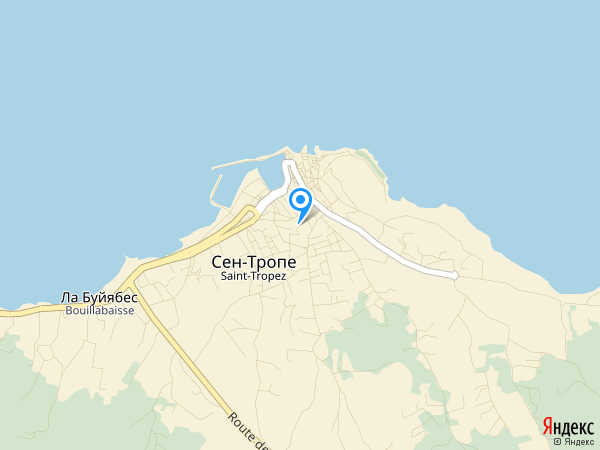
\includegraphics[width=400px]{map}}
	\fbox{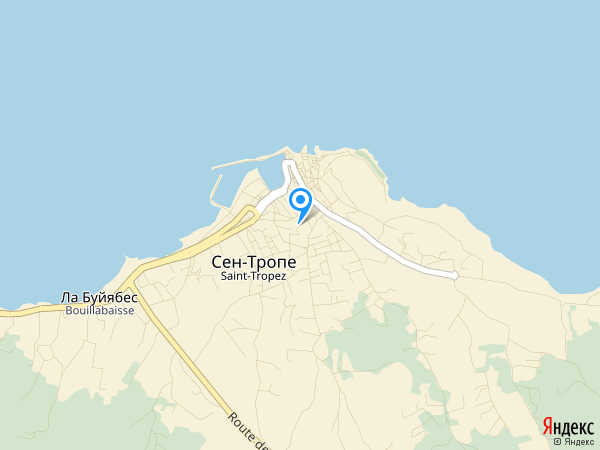
\includegraphics[width=0.9\textwidth]{map}}
	%		\fbox{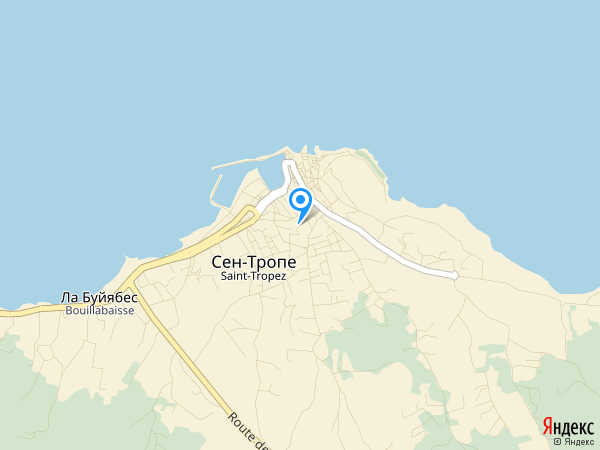
\includegraphics[width=650px]{map.png}}
	\caption{Обзорная карта района работ}
\end{figure}
Наблюдается общее понижение рельефа в~северо-восточном направлении, где присутствуют крупные болота и~озера. Абсолютные отметки колеблются от 37~м на~северо-востоке (оз. Леушинский Туман) до~330~м (гора Известковая) на~юго-западе, относительные превышения составляют в~среднем 50 -- 100~м (до 50~м в~восточной части). Крутизна склонов составляет обычно 6 -- 10\degree, редко до~20\degree.
Климат континентальный, среднегодовая температура около 0 \degree С. Средняя температура декабря и~января от  -- 10 до~ -- 17 \degree С (минимальная  -- 52 \degree С).

Средняя температура июля от +16 до~+17\degree (максимальная +37 \degree С). Осадки в~июле и~августе составляют 360 -- 426~мм, а в~январе -- феврале  --  100 -- 200~мм.
Установление снежного покрова наблюдается в~ноябре. Почвы, промерзая местами до~1~м, оттаивают в~мае. Большая часть площади занята лесами; реликтовые леса состоят в~основном из~ели, пихты, кедра, сосны и~березы, а на~старых вырубках и~гарях преобладают березово-осиновые. в~южной части территории листа О-41 присутствуют фрагменты лесостепных ландшафтов, представленных разнотравьем с осиново-березовыми колками, в~северо-восточной части широко представлены залесенные и~открытые болота с преобладающим моховым покрытием. Значительная часть южной и~западной частей района работ представлена сельскохозяйственными угодьями, занятыми кормовыми, овощными и~злаковыми культурами. 

Речная сеть территории относится главным образом к~бассейну р. Обь  --  реки Исеть, Нейва, Реж, Тагил, Тура, Ляля, Лобва, Тавда, Конда, и~только несколько водотоков в~юго-западной части  --  к~бассейну р. Кама (реки Чусовая и~Уфалейка). Речные долины преимущественно широкие, хорошо проработанные, в~западной части отмечаются и~каньонообразные. Питание рек происходит за счет талых вод и~атмосферных осадков, в~меньшей степени  --  за счет подземных вод. Реки на~большей части площади не судоходны (за исключением рек Тавда и~Тура в~нижнем течении), наиболее крупные из~них пригодны для прохождения на~лодках. Ледостав начинается в~начале ноября, ледоход  --  во второй половине апреля, толщина льда достигает 1~м. Для нужд энергетики и~металлургического производства на~всех
главных реках западной и~южной частей площади созданы пруды.

\begin{figure}[h]
	\centering
	\fbox{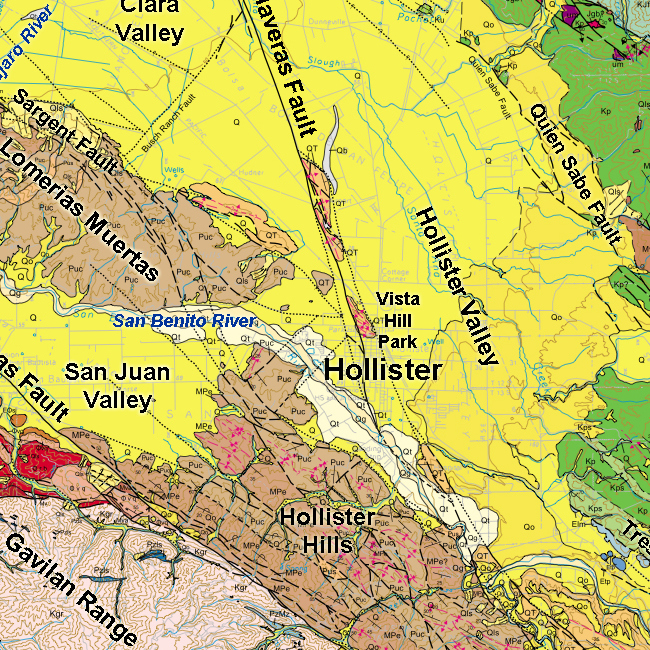
\includegraphics[width=0.9\textwidth]{geomap}}
%	\fbox{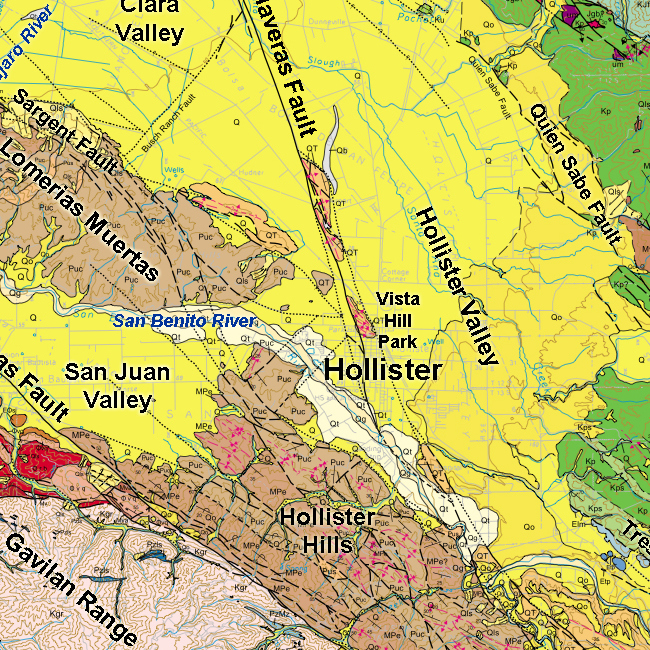
\includegraphics[width=400px]{geomap}}
	%		\fbox{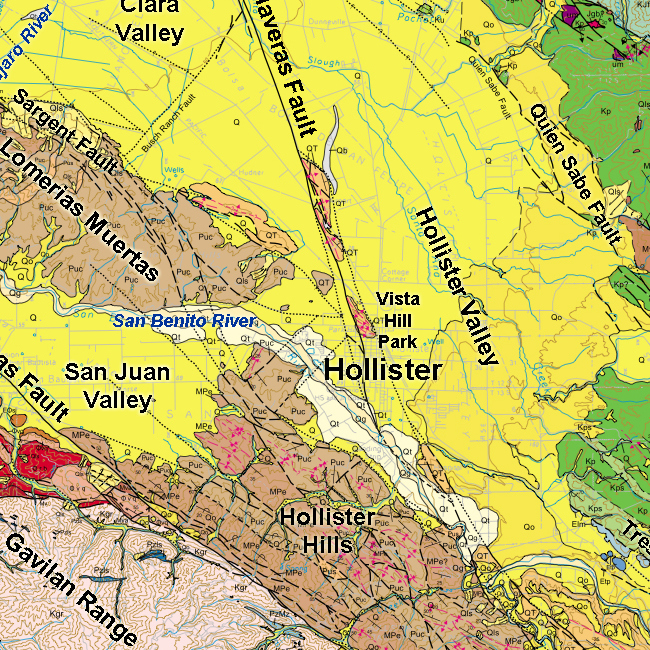
\includegraphics[width=650px]{geomap}}
	\caption{Геологическая карта района работ}
\end{figure}

\subsubsection{Геологические условия}
\txtGeology

\subsubsection*{Коры выветривания}
%Лист O-41
Коры выветривания относятся к~линейному и~площадному типам. Площадное распространение их определяется геоморфологическим строением, а тип коры  --  литологическим и~петрографическим составом пород субстрата. Наиболее хорошо от последующих размывов коры сохранились в~пределах депрессий, где наблюдается полный их профиль, а  мощность кор достигает 40  --  80~м. на~пологих склонах водоразделов и~холмов мощность кор от первых метров до~15 -- 20~м.

Линейные коры приурочены к~зонам контактов и~разрывных нарушений. к~линейному типу относятся и~контактово-карстовые коры, приуроченные к~тектоническим контактам силикатных пород и~карстующихся
известняков. Линейные коры распространяются на~глубину от нескольких десятков до~полутора сотен метров при протяженности от нескольких десятков до~нескольких сот километров. в~разрезе кор выветривания, независимо от состава материнских пород, отчетливо выделяются три зоны, связанные взаимными переходами (снизу вверх): 
\begin{itemize}
\item зона дезинтеграции (зона щебнистых и~дресвяно-щебнистых продуктов);
\item промежуточная зона зона глинисто-дресвянистых продуктов;
\item зона конечной гидратации (зона глинистых продуктов).
\end{itemize}


\textit{Зона дезинтеграции} характеризуется начальным выветриванием с образованием щебенистого или щебнисто -- дресвянистого элювия и~появлением в~породах гидрохлорита. 

В \textit{зоне промежуточных продуктов} увеличивается содержание гипергенных минералов: гидрохлорита, гидрослюды и~каолинита. 

\textit{Зона конечной гидратации} представлена пестроцветными, буроватыми, желтоватыми, зеленовато - серыми или темно - зелеными, часто структурными, глинами гидро\- слюдисто - каолинитового, гидрослюдисто - монтмориллонитового состава, нередко с галлуазитом, гидрослюдой, гиббситом, иногда алунитом; в~корах по~гранитоидам преобладают каолинит и~кварц, а в~корах по~ультрамафитам широко развиты нонтронит и~флогопит. Минералы тяжелой фракции представлены в~основном пиритом, сидеритом, лимонитом, мартитом, лейкоксеном. Вещественный состав кор выветривания обусловлен преобладанием одного из~двух минералого - геохимических типов  --  ферритно-сиаллитного, развитого по~породам основного состава, и~сиаллитного, характерного для пород среднего и~кислого составов.

\subsubsection*{Четвертичные образования}
%Лист O-41
Четвертичные образования имеют широкое распространение на~площади листа. Они представлены генетическими типами: флювиальными --- аллювий, лимний, лимноаллювий, палюстрий, лимнопалюстрий; субаэральными --- элювий, делювий, элювиоделювий, эолий, лессоиды; ледниковыми --- гляциалий, флювиогляциалий, лимногляциалий. в~речных долинах превалируют аллювиальные и~лимноаллювиальные отложения, мощность которых 10 -- 15~м в~верхнем течении и~30 -- 40 до~60~м -- в~нижнем. на~междуречьях широко распространен лимний в~озерных ваннах и~понижениях палеорельефа мощностью 5 -- 10 до~35~м, а также образования субаэрального и~палюстринного происхождения, мощность которых невелика --- 
от 2 -- 3 до~8~м. Ледниковые образования развиты локально в~северо-западном углу планшета и~имеют изменчивую мощность от 5 -- 10 до~25~м.
Возраст образований определен на~основании биостратиграфических данных с учетом палеомагнитных исследований и~радиоуглеродных датировок, а также в~соответствии со схемами стратиграфии Урала и~утвержденными легендами.

\subsubsection{Гидрогеологические условия}
%Лист O-41
%\textbf{Трещинные воды}. Уральская сложная гидрогеологическая складчатая область располагается в пределах орографически выраженного одноименного горно - складчатого сооружения. Основными коллекторами подземных вод являются трещиноватые породы коренного субстрата. Мощность зоны региональной трещиноватости составляет в среднем 30 – 100 м. Минимальные значения (20 – 30 м) присущи корам выветривания интрузивных пород; максимальные (60 – 100 м) – карбонатным породам; средние (40 – 60 м) – эффузивно-осадочным и метаморфическим комплексам. Помимо трещин выветривания широко развиты локальные линейные трещинные зоны высокой проницаемости и водоотдачи, связанные с проявлениями дизъюнктивной тектоники и контактами разнородных пород. Подземные воды региональной трещиноватости обычно гидравлически взаимосвязаны, имеют безнапорный характер и образуют небольшие бассейны с интенсивным
водообменном. В вертикальном разрезе фильтрационные свойства пород зоны выветривания неоднородны. По характеру их изменения зона разделяется на три части. В верхней (10 – 20 м), где широко представлены глины или суглинки элювиальной коры выветривания, водопроницаемые свойства очень низки; особенно широко коры распространены на площади Зауральского пенеплена. Средняя часть эрозионной зоны отличается наибольшей активностью, сильной степенью трещиноватости и высокой пористостью (от 1 до 7 \%). В нижней части размеры трещин весьма незначительны, и водоотдача пород практически отсутствует.

\textit{Водоносная зона трещиноватости позднепалеозойских интрузивных кислых и средних пород} ($\gamma PZ_3$) связана с массивами гранитов, гранодиоритов, плагиогранитов, диоритов. Региональная зона выветривания на этих массивах не превышает 15 – 20 м, зеркало подземных вод в сглаженной форме повторяет современный рельеф. Водоносность зоны крайне неравномерна: в центральных частях массивы практически безводны; по периферии (в приконтактовых частях с другими породами) водоносность возрастает до 0,2 – 0,3 л/с. В частности в тектонических и приконтактовых зонах позднепалеозойского Верхисетского гранитного массива отдельные скважины имели дебит до 7,0 л/с при удельном дебите 2,4 л/с, в центре массива оставаясь безводными. Минерализация вод – в пределах 0,08–0,5 г/дм\textsuperscript{3}; по составу преобладают гидрокарбонатные  кальциево-магниевые.

Гранодиориты и плагиограниты становятся более водоносными за счет секущих позднепалеозойских даек и жил «обновленных», к тому же тектоническими движениями создавшими условия для локализации трещинно-жильных вод в зоне выветривания. В окраинных частях Сысертского массива гранодиоритов и плагиогранитов дебиты скважин изменяются от 1,5 до 10,0 л/с при удельных дебитах 0,1 – 8,0 л/с. В центральной части (где нет жильных тел) в маломощной зоне выветривания дебиты скважин не превышают 0,3 – 0,5 л/с при удельных дебитах 0,001–0,01 л/с. Ближе к периферии фиксируютя мелкие источники с расходом 0,1 – 0,2 л/с. По минерализации и химическому составу воды аналогичны развитым в гранитных массивах. 

В целом питание подземных вод Большеуральского бассейна сезонное, за счет инфильтрации атмосферных осадков в теплый период года. Зеркало его вод в сглаженной форме повторяет основные элементы рельефа. На склонах и уплощенных водоразделах уровни воды залегают на глубинах 5 – 20 м, на хребтах и локальных возвышенностях – до 30 – 50 м. Сравнительно глубокая расчлененность дневной поверхности, особенно в районах приподнятых горных массивов, обеспечивает хорошие условия дренирования водоносных зон речной сетью. Разгрузка вод идет преимущественно вдоль долин рек, а также может быть приурочена к локальным трещинным зонам. Дебиты родников, в зависимости от величины водосборной площади, варьируют от долей до многих десятков литров в секунду.

Эксплуатационные ресурсы Большеуральского бассейна связываются преимущественно с крупными карбонатными массивами среднего и верхнего палеозоя и тектонически активными зонами разломов, на которых возможна организация водозаборов с дебитом 100 – 1000 л/с. На остальных водоносных зонах трещиноватости возможен каптаж подземных вод по отдельным кустам скважин с дебитами от 10 до 30 л/с. Ресурсы порово-пластовых вод Иртыш-Обского бассейна связаны преимущественно с опоковым горизонтом палеоцена, мощность обводненной толщи которого 3 – 4 м на западе и до 50 м на востоке. На придолинных участках некоторые водозаборы из него имеют производительность до 50–100 л/с.

Несмотря на значительное количество водоносных горизонтов на изученной площади, наиболее промышленные и обжитые районы Урала испытывают недостаток в водообеспеченности из-за неравномерного распределения ресурсов, а также в связи с невозможностью создания крупных водозаборов с высокой производительностью на локальных участках водоносных зон.

\hydrogeology

\begin{figure}[!h]
	\centering
	\includegraphics[height=1.0\textwidth]{\txtLegendFname}
%	\includegraphics[height=0.98\textheight]{\txtLegendFname}
%	\includegraphics[width=400px]{\txtLegendFname}
	\caption[Условные обозначения]{Условные обозначения к~геологической карте}
	\label{img:legend}
\end{figure}

\subsection{Результаты рекогносцировочных работ}
Рекогносцировочные работы, выполненные методом маршрутной съемки в~районе площадки проектируемого строительства, позволили получить следующие результаты:

\txtRecog

\subsection{Камеральные работы}
На основе выполненных камеральных работ установлено:
\txtCamer

\section{Рекомендации}
\txtRecommend


\end{document} % конец документа
